%
%	 untitled
%
%	 Created by Jesper Josefsson on 2011-10-10.
%	 Copyright (c) 2011 __MyCompanyName__. All rights reserved.
%
\documentclass[]{article}

% Use utf-8 encoding for foreign characters
\usepackage[utf8]{inputenc}

% Setup for fullpage use
\usepackage{fullpage}

% Uncomment some of the following if you use the features
%
% Running Headers and footers
\usepackage{fancyhdr}

% Multipart figures
%\usepackage{subfigure}

% More symbols
\usepackage{amsmath}
\usepackage{amssymb}
\usepackage{latexsym}

% Surround parts of graphics with box
\usepackage{boxedminipage}

% Package for including code in the document
\usepackage{listings}

% If you want to generate a toc for each chapter (use with book)
\usepackage{minitoc}

% This is now the recommended way for checking for PDFLaTeX:
\usepackage{ifpdf}

%\newif\ifpdf
%\ifx\pdfoutput\undefined
%\pdffalse % we are not running PDFLaTeX
%\else
%\pdfoutput=1 % we are running PDFLaTeX
%\pdftrue
%\fi

\ifpdf
\usepackage[pdftex]{graphicx}
\else
\usepackage{graphicx}
\fi
\title{SSY080 \\ Inlämningsuppgift}
\author{
Linus Oleander - 880613 - 4873 \\
Jesper Josefsson - 860409 - 5276 
}

\date{2011-10-10}

\begin{document}

\ifpdf
\DeclareGraphicsExtensions{.pdf, .jpg, .tif}
\else
\DeclareGraphicsExtensions{.eps, .jpg}
\fi

\maketitle

\section{Bakgrund}
Uppgiften går ut på att genomföra ett antal experiment gällande generering och behandling av signaler med Matlab.

\section{Generering av fyrkantsvåg med hjälp av Fourierserie - (3.1)}
\subsection{Fourierkoefficienter} % (fold)
\label{sub:fourierkoefficienter}
Den första uppgiften var att ta fram ett slutet uttryck för Fourierseriekoefficienterna $A_k$ och $B_k$.\\
Vi använde följande samband:\\
\begin{align*}
	C_k &= \frac{1}{T} \int_0^T \! x(t) e^{-jk\omega_0 t}\, \mathrm{d} t =\\
			&= \frac{1}{T} \left(
						\int_0^{\frac{T}{2}} \! e^{-jk\omega_0 t}\, \mathrm{d} t
						- \int_{\frac{T}{2}}^T \! e^{-jk\omega_0 t}\, \mathrm{d} t \right) =\\
			&= \frac{1}{-jk\omega_0 T} \left(
						\left[e^{-jk\omega_0 t}\right]_0^{\frac{T}{2}}
						- \left[e^{-jk\omega_0 t}\right]_{\frac{T}{2}}^T
					\right) = \\
			&= \left[
					\omega = \frac{2\pi}{T} \Rightarrow \frac{\omega_0 T}{2} = \pi ,\;	\omega_0 T = 2\pi
				\right] = \\
			&= \frac{1}{-jk\omega_0 T} \left(
					2e^{-jk\pi} - e^{-jk2\pi} - 1
				\right) = \\
			&=	\left[
					\begin{array}{ll}
						2e^{-jk\pi} &=
							\left\{
								\begin{array}{ll}
									-2	& ,k\text{ udda} \\
									2 & ,k\text{ jämn} 
								\end{array}
							\right. \\
						e^{-jk2\pi} &= 1
					\end{array}
					\right] = \\ \\
			&= \left\{ \begin{array}{ll}
						\frac{-4}{-jk2\pi} = \frac{2}{jk\pi} = -\frac{2j}{k\pi}&,k\text{ udda} \\
						0 &,k\text{ jämn}
					\end{array} \right.\\
	A_k &= C_k - C_{-k} = -\frac{2i}{k\pi} + \frac{2i}{k\pi} = 0\\
	C_k &= \frac{1}{2}(A_k - iB_k) \Rightarrow B_k = 2iC_k = \frac{4}{k\pi}\\
\end{align*}
% subsection fourierkoefficienter (end)

\subsection{Generering av fyrkantsvåg} % (fold)
Vi använder Fourierkoefficienterna för att generera en fyrkantsvåg i matlab med hjälp av definitionen av Fourierserien på trigonometrisk form: 
\[
	x(t) = A_0 + \sum\limits_{k=1}^\infty [A_k cos(k\omega_0 t) + B_k sin(k\omega_0 t)] \\
\]

Koden blir som nedan:

\begin{verbatim}
T = 2;
w=2*pi/T;
M=200;
t=T*(0:M-1)/M;
y = @(t) 0;
bs = [];
for k=1:100
		ck = -(mod(k, 2))*((1i*2)/(pi*k));
		cminusk = -(mod(k, 2))*((1i*2)/(pi*(-k)));
		ak = ck + cminusk;
		bk = 2i*ck;
		bs = [bs bk];
		y = @(t) y(t) + ak*cos(k*w*t) + bk*sin(k*w*t);
end
\end{verbatim}

För fyrkantsvåg, se figur 1.
% subsection generering_av_fyrkantsvåg (end)

\section{Linjära system och sinusar (3.2)} % (fold)
\subsection{Konstruering av givet system} % (fold)
\label{sub:konstruering_av_givet_system}
Vi konstruerar först ett LTI-system med ett frekvenssvar $G(j\omega)$ som är givet i uppgiften. \\
Därefter plottar vi det i frekvensdomänen samt studerar dess poler och nollställen - figur 2 och 3.
\begin{verbatim}
% num = (s + 0.1)(s + 10) = s^2 + 10.1s + 1
% den = (s + 1)(s^2 + s + 9) = s^2 + 2s^2 + 10s + 9
num = {[1 10.1 1]};
den = {[1 2 10 9]};
H = tf(num, den);
bode(H)
title('Bode for H');
% pzmap(H);
% sgrid
% grid on
\end{verbatim}

I Bode-diagrammet framkommer systemets påverkan på olika frekvenserkomponenter i insignalen. I det övre diagrammet kan vi se systemets amplitudpåverkan. Till exempel förstärks komponenter med vinkelfrekvens $\omega = 3$ med ungefär $10dB$. \\
I det undre diagrammet ser vi systemets faspåverkan. Till exempel får komponenter med vinkelfrekvensen $\omega = 3$ en förskjutning på ungefär $-100^\circ$.

% subsection konstruering_av_givet_system (end)

\subsection{Insignaler skapas och körs genom systemet} % (fold)
\label{sub:insignal}

Tre insignaler skapas. Dessa är sinusformade signaler med vinkelsfrekvenserna $\omega = [1,2,3]$. \\
Därefter används matlab för att simulera systemets påverkan på signalerna. In- och utsignal plottas, se figur 4-6.

\begin{verbatim}
N = 8192;
f = 100;
Ts = 1/f;
Tmax = (N-1)*Ts;
t= 0:Ts:Tmax;
Xs = ones(3,N);
Y = ones(3,N);
index = 1;
for w=[1 3 5],
    x = sin(w*t);
    Xs(index,:) = x;
    [y, t] = lsim(H,x,t);
    Y(index,:) = y;
    index = index +1;
end
plot(t,Y(1,:), 'b',t, Xs(1,:),'r')
title('In and out signals for w=1');

% plot(t,Y(2,:), 'b',t, Xs(2,:),'r')
% title('In and out signals for w=3');

% plot(t,Y(3,:), 'b',t, Xs(3,:),'r')
% title('In and out signals for w=5');
\end{verbatim}
Man kan se att utsignalerna har samma periodtid som insignalerna. Man kan också se att det har skett amplitudpåverkan samt faspåverkan.
Med hjälp av evalfr kan vi bestämma systemets teoretiska amplitud- och faspåverkan:
\begin{verbatim}
>> abs(evalfr(H,1i))
ans =
    0.8858
>> abs(evalfr(H,3i))
ans =
    3.3033
>> abs(evalfr(H,5i))
ans =
    0.6541
>> angle(evalfr(H,1i))*180/pi
ans =
   37.8750
>> angle(evalfr(H,3i))*180/pi
ans =
  -56.7750
>> angle(evalfr(H,5i))*180/pi
ans =
 -125.9168
\end{verbatim}

Ur detta kan man läsa att förhållandet $y(t) = g(\omega) sin(\omega t + \phi (\omega))$ stämmer.
% subsection insignal (end)

\section{Periodiska insignaler och DFT}
\subsection{DFT för matlabs fyrkantsvåg} % (fold)
Först plottades matlabs fyrkantsvåg - se figur 7.
Vi konstaterar att funktionen är udda eftersom $f(-x) = -f(x)$. Detta syns dåligt i diagrammet, eftersom vågen genererades med utgångspunkt $t = 0$. \\
Därefter plottades frekvenssvaret för matlabs fyrkantsvåg, se figur 8.
\begin{verbatim}
x = square(t);
% plot(t,x);

k = 0:(N-1);
wk = 2*pi*fs*k/N;
X = fft(x,N);

plot(wk, abs(X))
\end{verbatim}


Sedan användes ett antal uttryck för att räkna ut de teoretiska Fourierkoefficienterna. Det empiriskt utkomna koefficienterna räknades ut med matlabrutinen evalfr. \\

\begin{tabular}{|c||ccc|}
  \hline
  \multicolumn{4}{|c|}{Fourierkoefficienter för fyrkantsvåg} \\
  \hline
  Teoretiska & 1.2732 & 0.4244 & 0.2546\\
  \hline
  Empiriska & 1.2702 & 0.4154 & 0.2398\\
  \hline
\end{tabular}
% subsection dft_för_matlabs_fyrkantsvåg (end)
\subsection{Systemet appliceras på fyrkantsvågen} % (fold)
\label{sub:systemet_appliceras_pa_fyrkantsvagen}
Det tidigare angedda systemets påverkan på fyrkantsvågen beräknas med hjälp av rutinen lsim.\\
Fourierkoefficienterna för utsignalen y beräknas med hjälp av givna ekvationer och tas även fram empiriskt med hjälp av matlabrutinen evalfr. \\
Till sist plottas y i frekvensplanet - se figur 9.\\
Där framgår det att $\omega = 1$ är lite förstärkt, $\omega = 3$ är kraftigt förstärkt, och $\omega = 5$ är kraftigt sänkt. \\ \\
\begin{tabular}{|c||ccc|}
  \hline
  \multicolumn{4}{|c|}{Fourierkoefficienter för fyrkantsvåg efter system G} \\
  \hline
  Teoretiska & 1.1279 & 1.4020 & 0.1666\\
  \hline
  Empiriska & 1.1023 & 1.3378 & 0.1513\\
  \hline
\end{tabular}
% subsection systemet_appliceras_på_fyrkantsvågen (end)
% section linjära_system_och_sinusar_3_2_ (end)
\section{Notch-filter}
\subsection{Nollställen} % (fold)
\label{sub:konstruktion_av_taljar_och_namnarpolynom}
Ett polynom för ett notch-filter ska konstrueras. \\
Nollställen väljs för $\omega = [1,5,7,9]$ samt $\omega = 0$: \\
\[
  \text{täljarpolynom} = s(s - 1)(s + 1)(s - 5)(s + 5)(s - 7)(s + 7)(s - 9)(s + 9)
\]
Därefter plottas frekvenssvaret - se figur 10.
\begin{verbatim}
  roots = [0 -1i 1i -5i 5i -7i 7i -9i 9i];
  num = poly(roots);
  sys = tf(num, 1);
  bode(sys)
\end{verbatim}
\subsection{Poler} % (fold)
\label{sub:poler}
Polerna väljs enligt $p = -4$. Antalet bestämmer dämpningen av högre frekvenser. Empiriska test visar att det behövs i storleksordningen 21 poler för att uppnå $60dB$ dämpning för $\omega > 9$. \\
\begin{verbatim}
proots = -4*ones(1,21);
den = poly(proots);
\end{verbatim}
\subsection{Förstärkning} % (fold)
\label{sub:forstarkning}
Förstärkningen ska normalisera till $0dB$ för $\omega = 3$. Det görs genom att man lägger till ett nollställe vid $\omega = 3$ som bildar den förstärkande faktor som behövs: \\
\[
  (3i - x) = 1/(\text{skalfaktor före korrigering})
\]
Skalfaktorn före korrigering räknas med med evalfr: \\
\begin{verbatim}
evalfr(sys, 3i)
\end{verbatim}

Den slutgiltiga koden blir: \\

\begin{verbatim}
roots = [0 -1i 1i -5i 5i -7i 7i -9i 9i 4.31165e8];
num = poly(roots);
proots = -4*ones(1,21);
den = poly(proots);
sys = tf(num,den);
\end{verbatim}

\subsection{Slutgiltiga filterresultat} % (fold)
\label{sub:slutgiltiga_filterresultat}
Se figur 11.
% subsection slutgiltiga_filterresultat (end)

% subsection förstärkning (end)
\section{Figurer} % (fold)
\label{sec:figurer}
\begin{figure}[hbt]
  \centering
  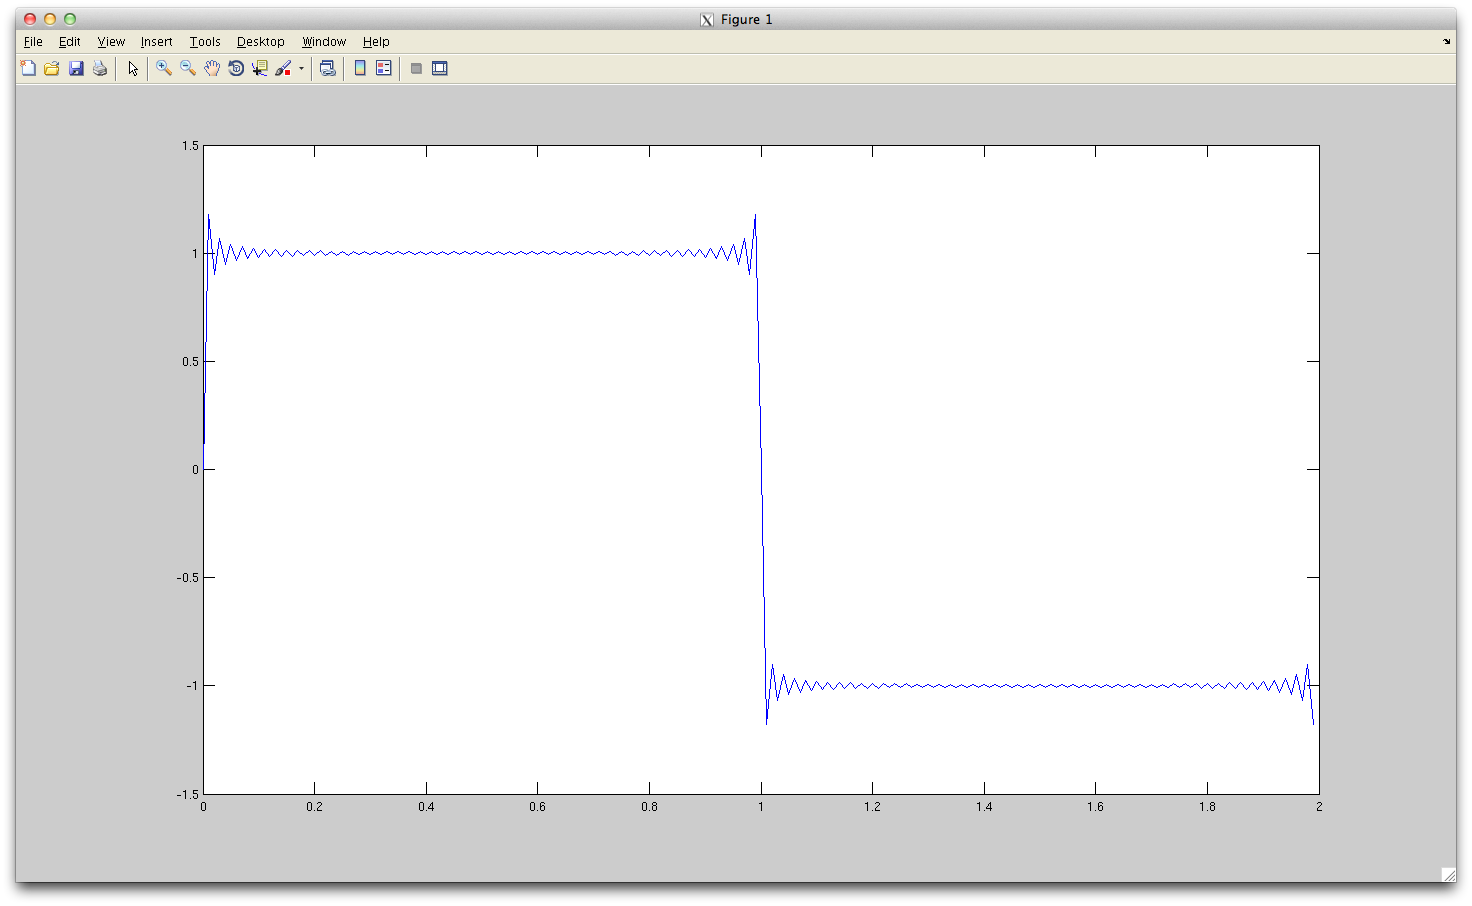
\includegraphics[width=15.0cm]{square.png}
  \caption{Vår fyrkantsvåg}
\end{figure}
\begin{figure}[hbt]
  \centering
  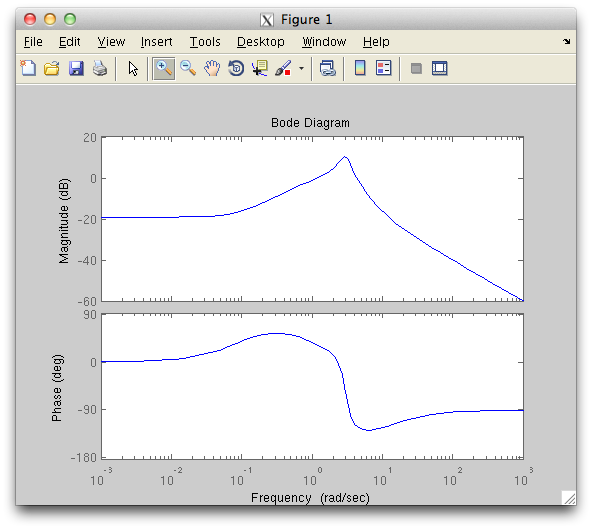
\includegraphics[width=15.0cm]{bode.png}
  \caption{Bode-diagram för $G(j\omega)$}
\end{figure}
\begin{figure}[hbt]
  \centering
  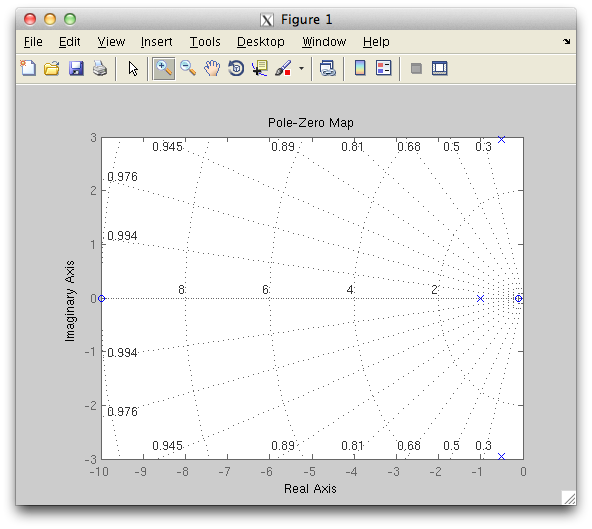
\includegraphics[width=15.0cm]{pzmap.png}
  \caption{pzmap}
\end{figure}
\begin{figure}[hbt]
  \centering
  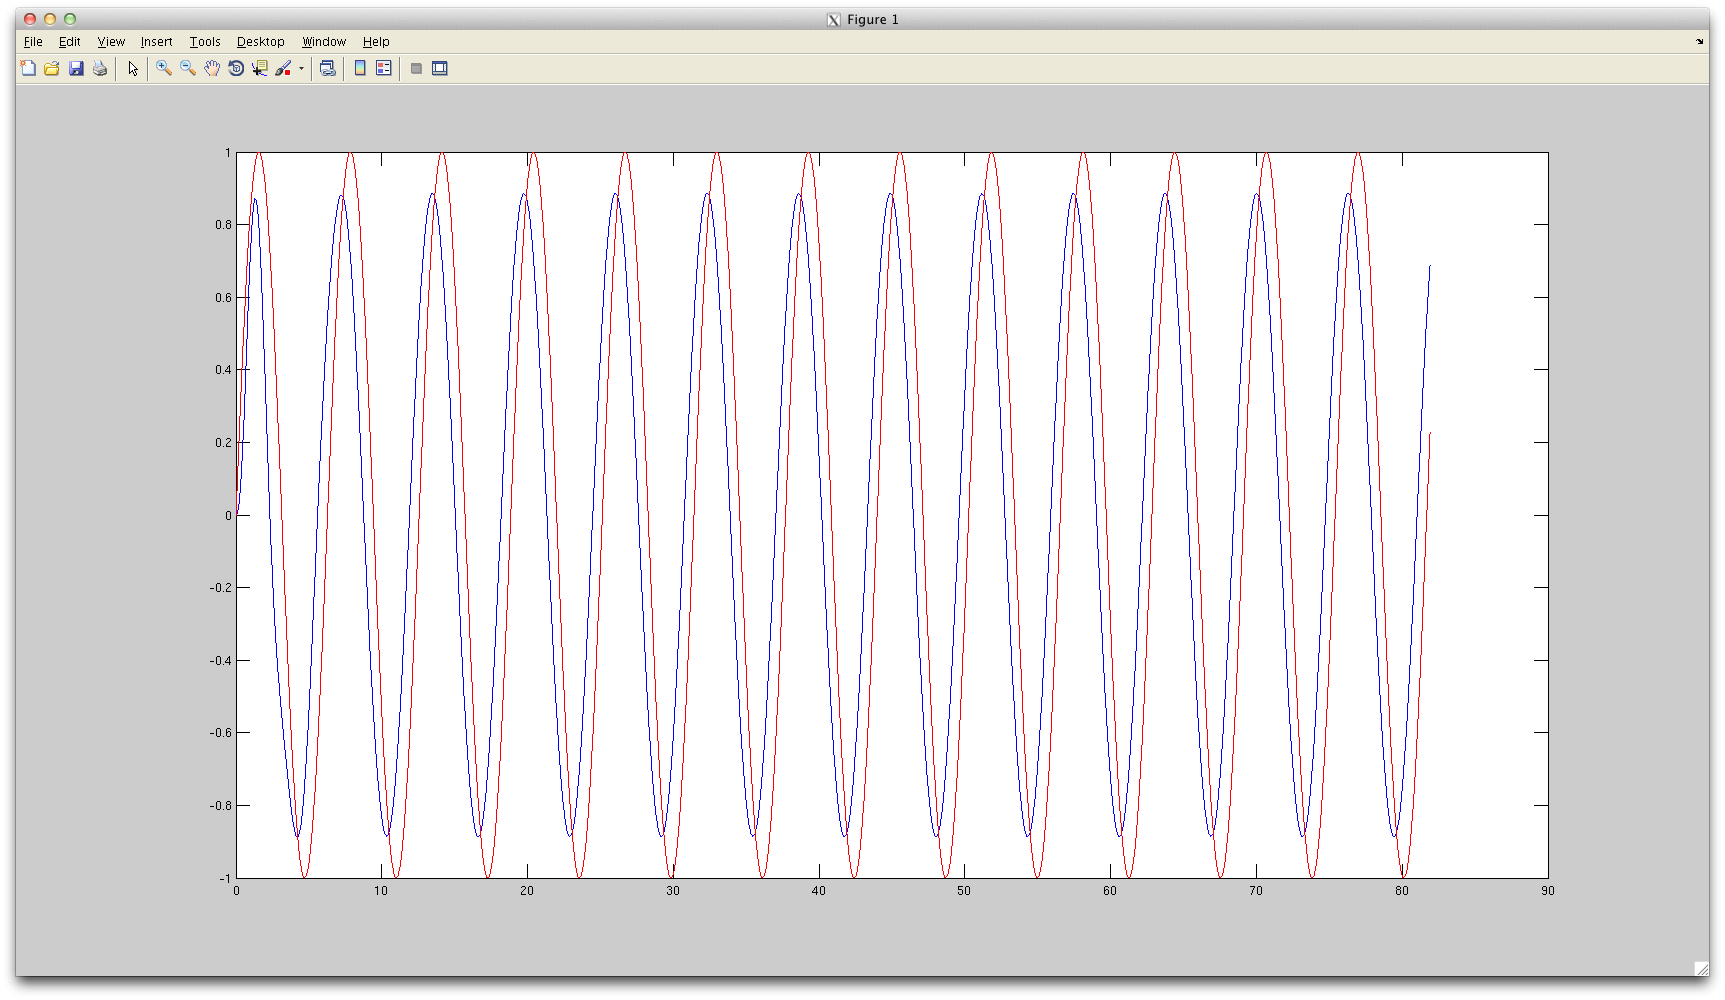
\includegraphics[width=15.0cm]{omega 1.png}
  \caption{$\omega = 1$}
\end{figure}
\begin{figure}[hbt]
  \centering
  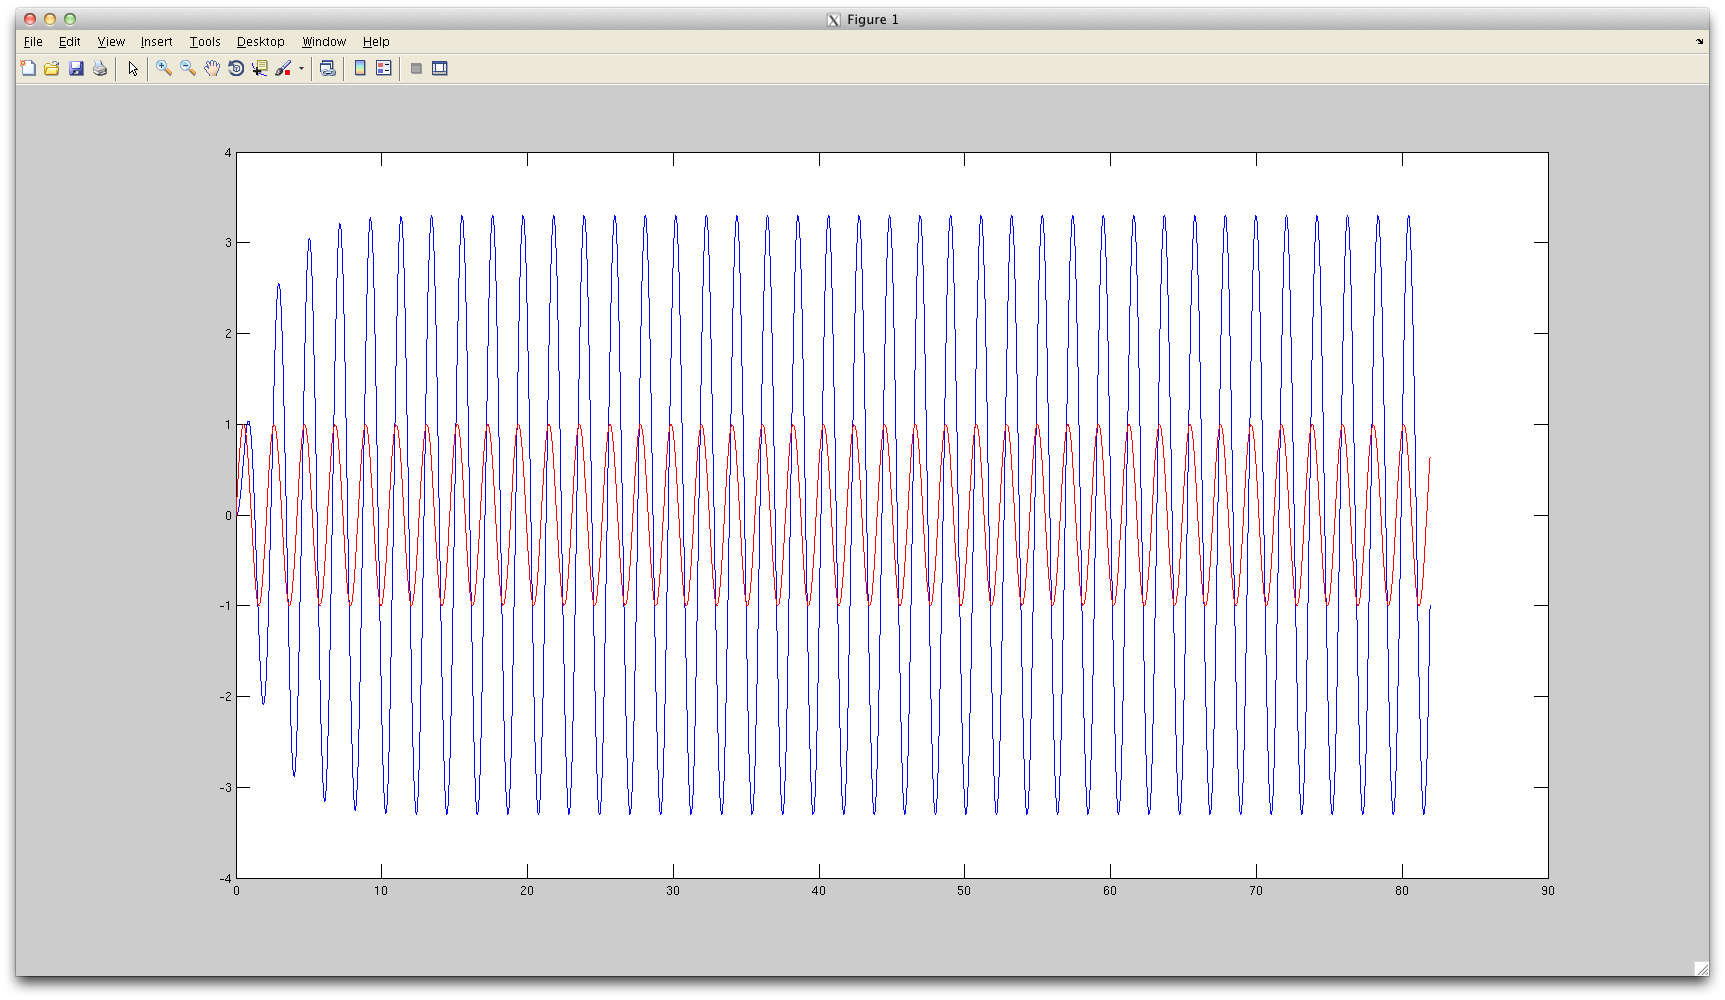
\includegraphics[width=15.0cm]{omega 3.png}
  \caption{$\omega = 3$}
\end{figure}
\begin{figure}[hbt]
  \centering
  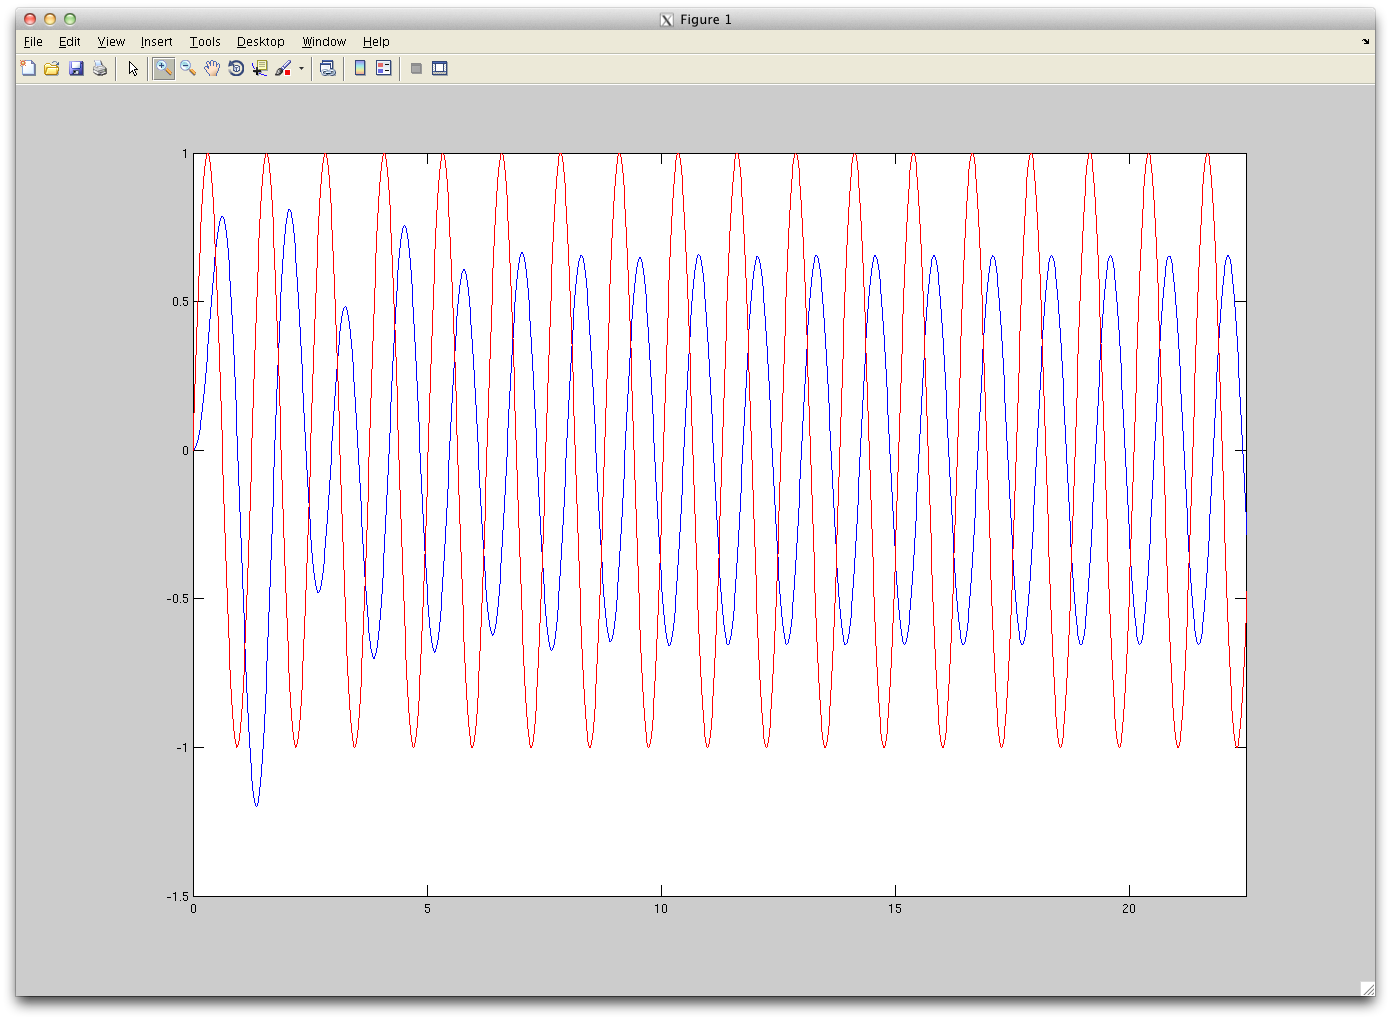
\includegraphics[width=15.0cm]{omega 5.png}
  \caption{$\omega = 5$}
\end{figure}
\begin{figure}[hbt]
  \centering
  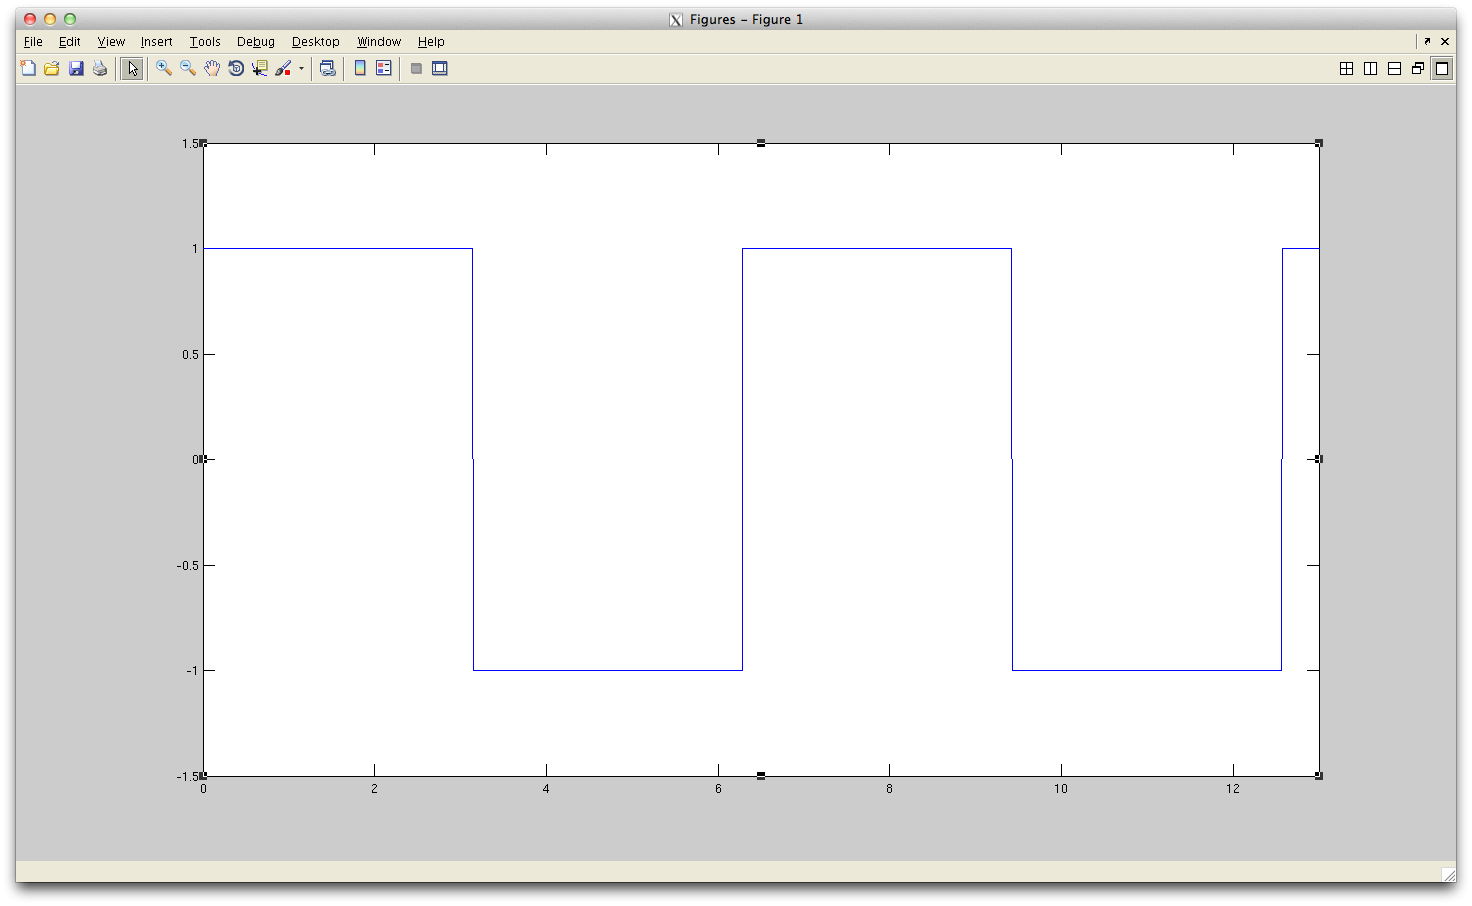
\includegraphics[width=15.0cm]{matlabsquare.png}
  \caption{Matlabs fyrkantsvåg}
\end{figure}
\begin{figure}[hbt]
  \centering
  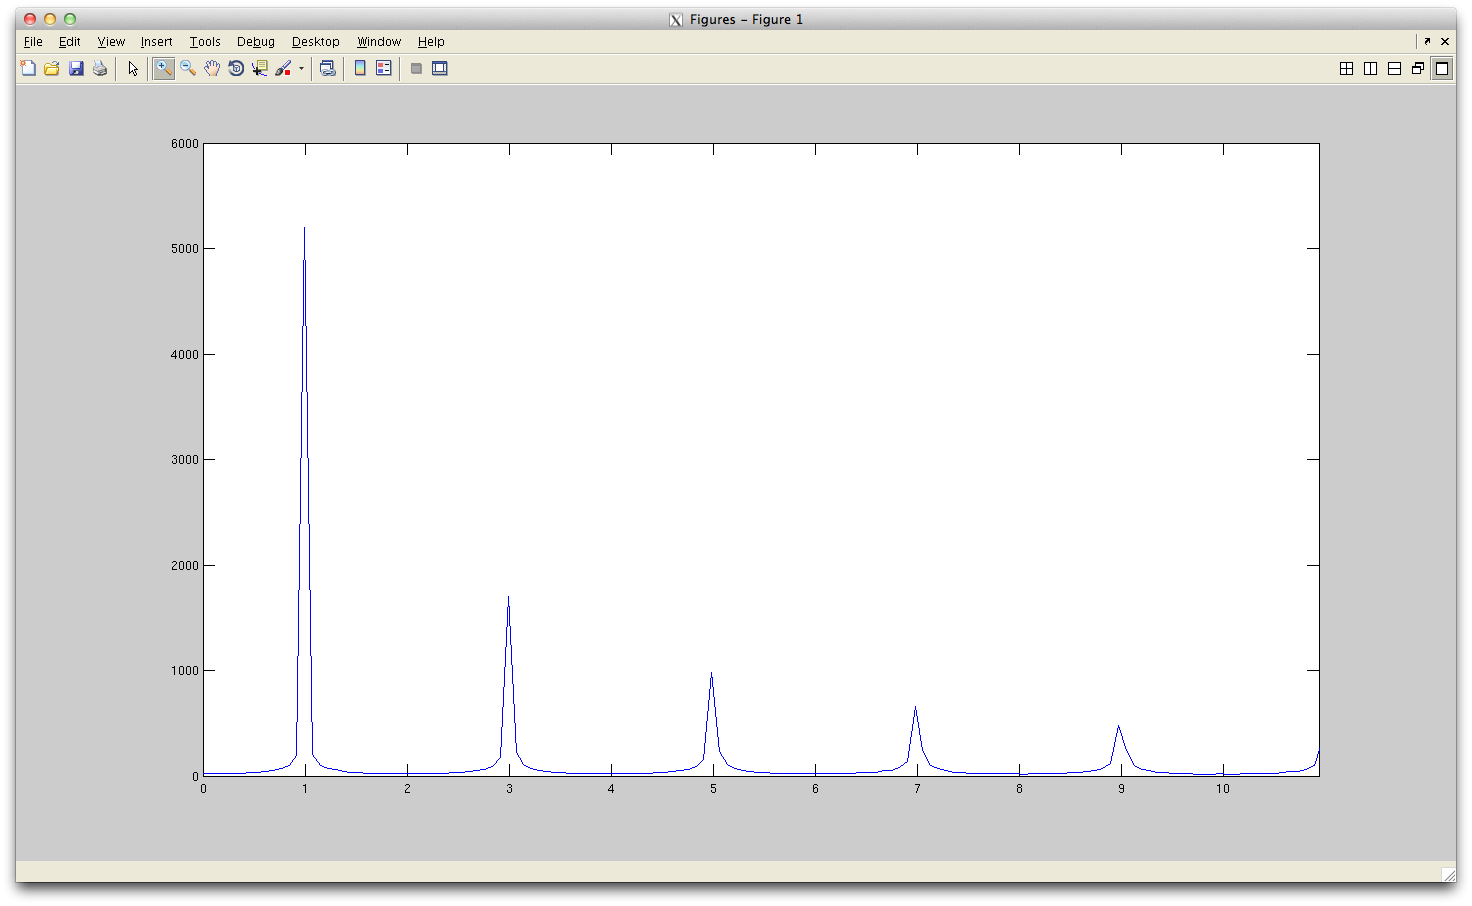
\includegraphics[width=15.0cm]{matlabsquaredft.png}
  \caption{DFT-transform av matlabs fyrkantsvåg}
\end{figure}
\begin{figure}[hbt]
  \centering
  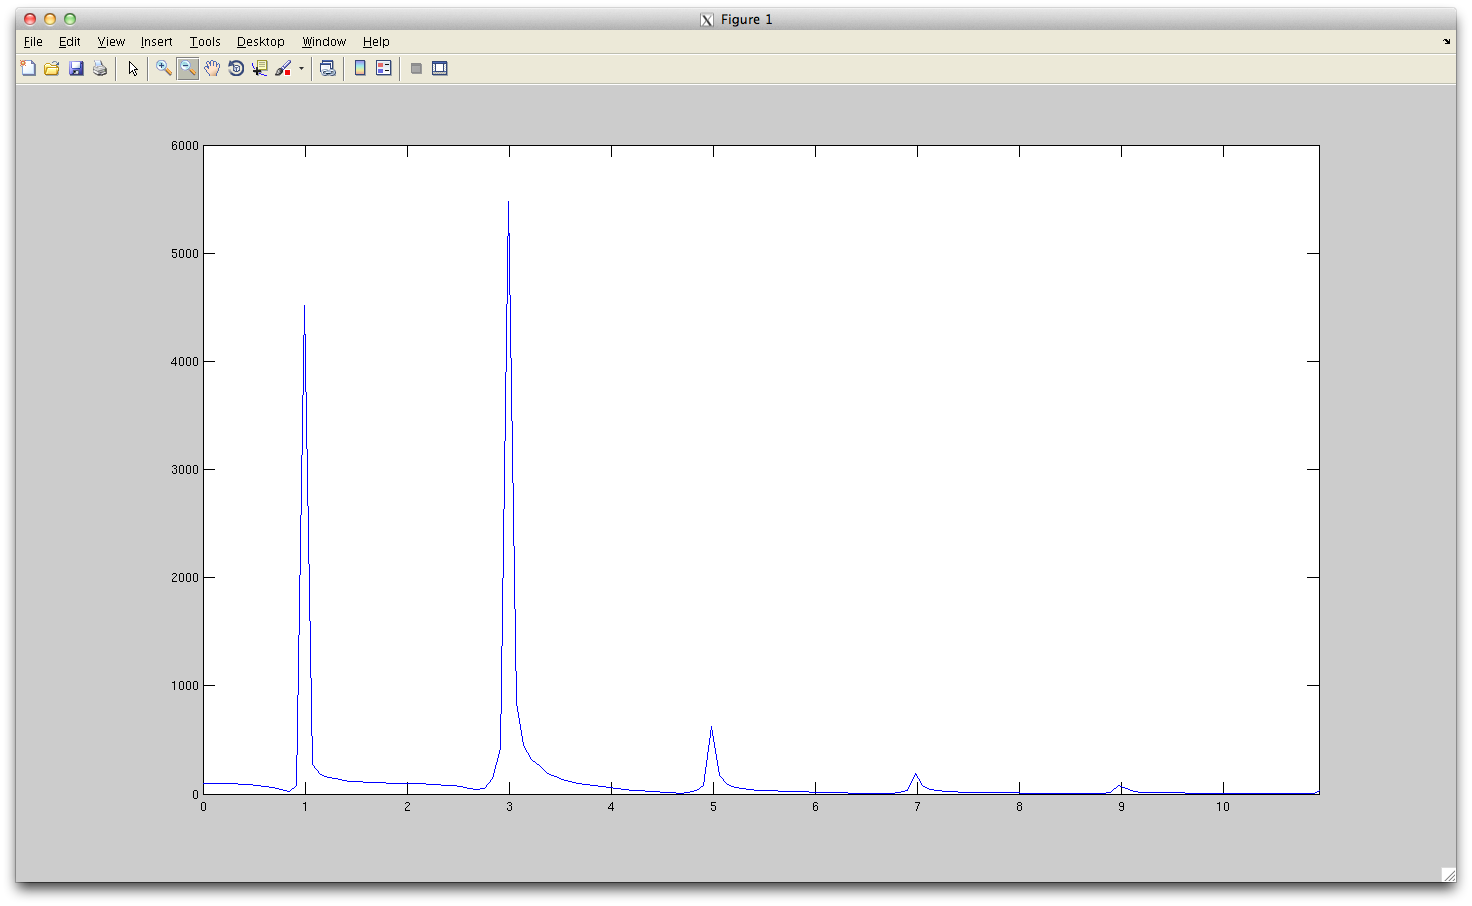
\includegraphics[width=15.0cm]{dftY.png}
  \caption{DFT-transform av fyrkantsvåg efter påverkan från system G}
\end{figure}
\begin{figure}[htb]
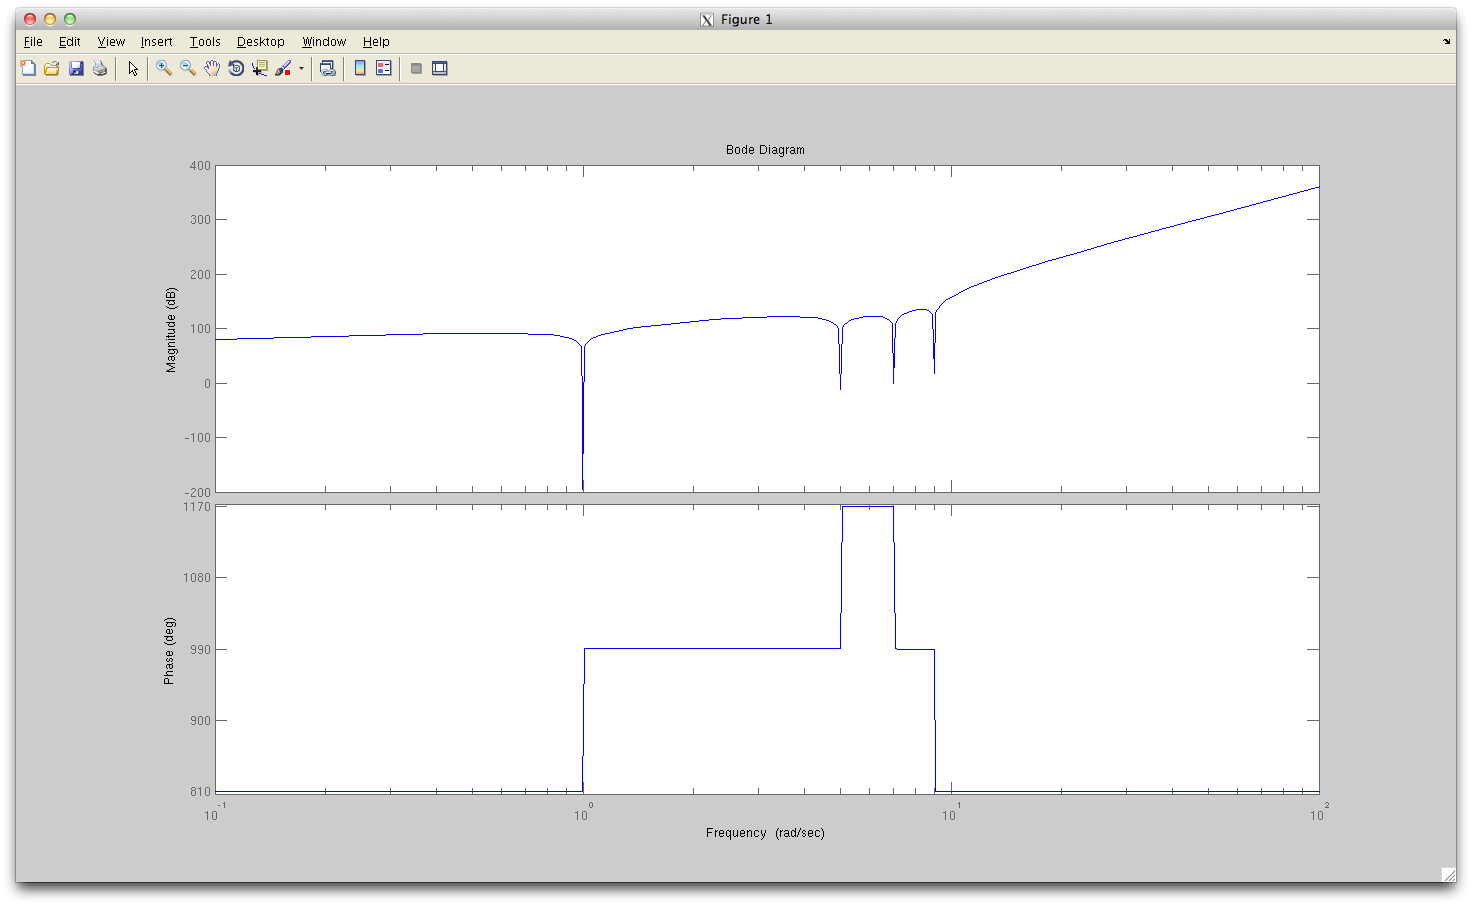
\includegraphics[width=15.0cm]{baranollst.png}
\caption{Notchfiler med endast nollställen}
\end{figure}
\begin{figure}[htb]
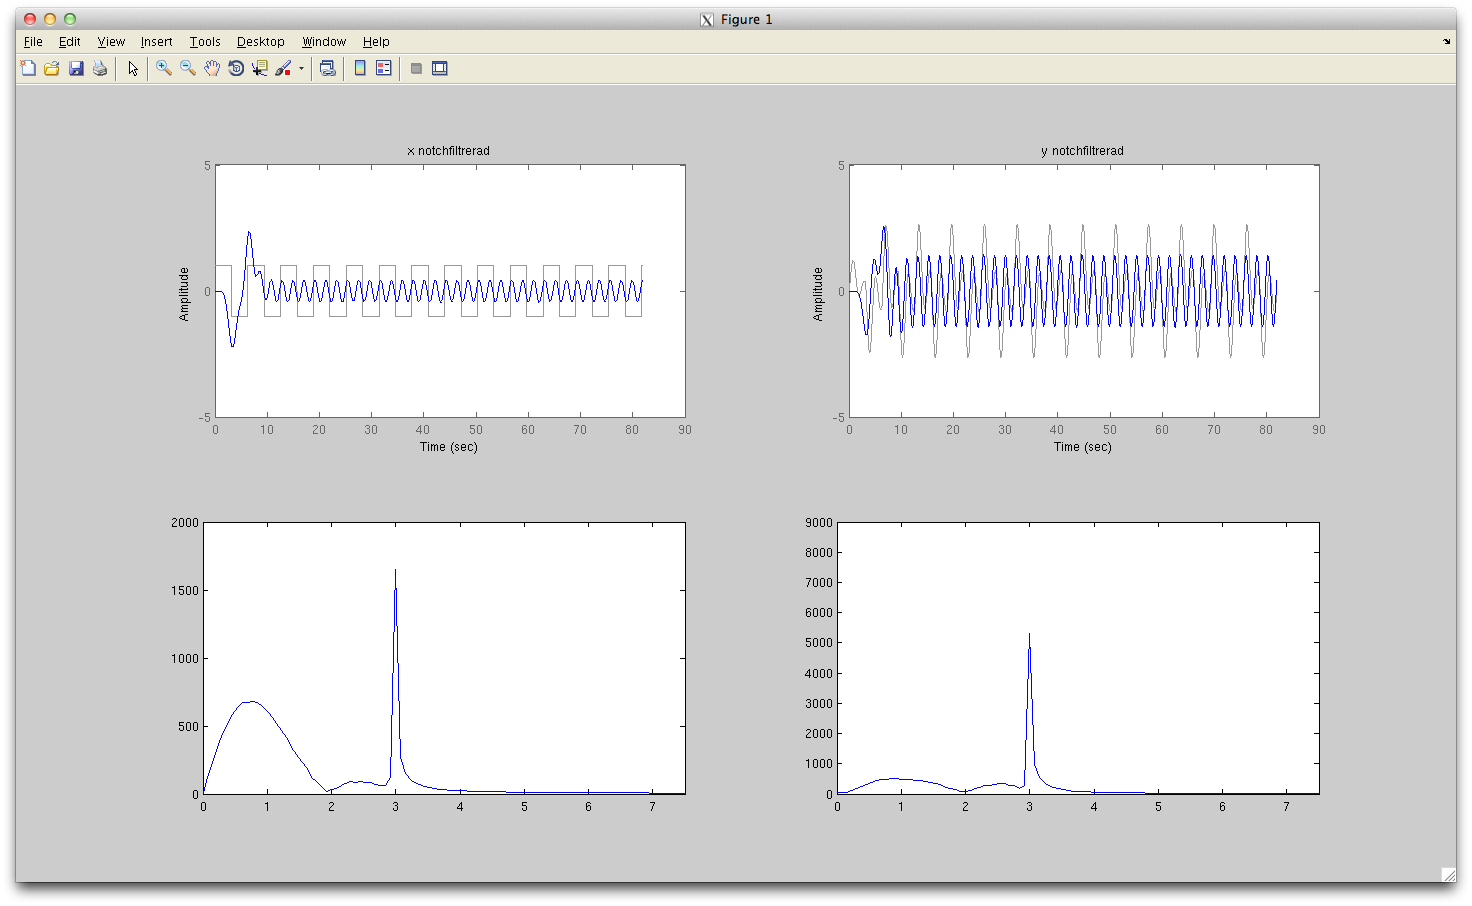
\includegraphics[width=15.0cm]{filterresultat.png}
\caption{Resultat efter notchfiltrering - x är fyrkantsvåg, y är fyrkantsvåg med påverkan av det givna systemet}
\end{figure}
% section figurer (end)
\bibliographystyle{plain}
\bibliography{}
\end{document}
